\begin{figure}[t]
\centering
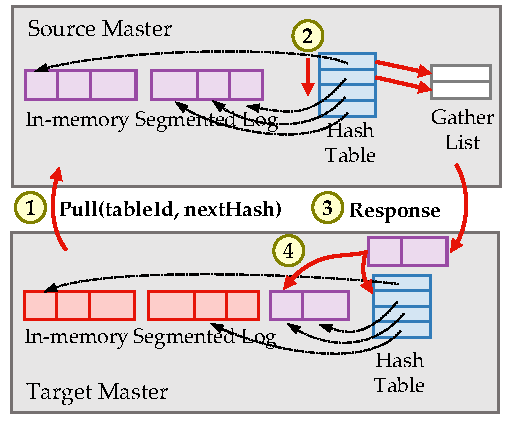
\includegraphics[width=0.70\columnwidth]{figures/rocksteady-overview.pdf}
\caption{Overview of Rocksteady \pulls. A \pull RPC issued by the target
    iterates down a portion of the source's hash table and returns a
    batch of records. This batch is then logically replayed by the
    target into its in-memory log and hash table.}
%\one The target issues pull requests
%to fetch batches of records from the source. \two The target copies the
%addresses of the next set of records into a DMA gather list. \three The
%gather list is posted to the NIC which DMAs records directly from the source
%log to the target. \four The target incoporates the received records into its own
%log and updates its hash table. Migration is pipelined and parallel;
%multiple pulls are in-flight at a time, and both the source and target
%adaptively process pulls on multiple cores.}
\label{fig:migration-overview}
\end{figure}
